\chapter{SaaS, le tecnologie che ne consentono la realizzazione}
Nel corso degli ultimi anni, con il proliferarsi delle piattaforme e dei servizi di Cloud Computing, sono nate e si sono sviluppate molte tecnologie per soddisfare le nuove esigenze e i nuovi requisiti appena visti che questa rivoluzione della fruizione del software ha comportato.

\section{Microservizi}
Un concetto fondamentale, di cui il Cloud Computing fa largamente uso, sono i mircoservizi. Cominciamo col darne una definizione abbastanza formale: "Lo stile architetturale a microservizi è un approccio allo sviluppo di una singola applicazione come insieme di piccoli servizi, ciascuno dei quali viene eseguito da un proprio processo e comunica con un meccanismo snello, spesso una HTTP API.(Martin Fowler)".

\paragraph{}
L'approccio è quello di dividere le funzionalità del sistema in più microservizi. Ad ogni microservizio corrisponde una necessità dell'utente. La filosofia di dividere il software in base alle responsabilità è già presente da tempo nell'ingegneria del software. Una suddivisione modulare del sistema in base ai casi d'uso dell'utente è già presente da tempo nell'Object Oriented Design, ma la novità apportata dai microservizi è che il sistema con essi risulta scomposto in realtà in piccoli servizi completamente indipendenti tra loro. Ogni microservizio si preoccupa infatti di risolvere un particolare problema del cliente, un unico scenario. La comunicazione tra i servizi avviene attraverso la rete al fine di garantire l'indipendenza tra i servizi ed evitare ogni forma di accoppiamento. Ogni microservizio, infatti, rappresenta un'entità separata che generalmente viene pubblicata come un modulo di una Platform as a Service.

\subsection{Il modello monolitico a layer }
Secondo il classico modello a layer le funzionalità vengono suddivise in base al grado di astrazione tra i vari livelli, usando delle tecnologie proprie di ogni livello. Questi sono separati a livello logico e comunicano tra di loro. Con questa architettura però, nonostante ci sia questa suddivisione a strati, il software risulta essere un unico sistema monolitico, sebbene molti componenti possano essere comunque riusabili.

\begin{figure}[h!]
	\centering
	
\includegraphics[width=\textwidth,keepaspectratio=true]{capitoli/imgs/disegnoMicrosMonol.png}
	\caption{Il modello monolitico e i microservizi}
\end{figure}

\subsection{Confronto tra l'architettura a microservizi e il modello monolitico}
La scelta di adottare uno o l'altro approccio viene dopo un'attenta analisi dei requisiti che il sistema deve soddisfare. In questo studio però va anche tenuto conto quanto le esigenze possano cambiare nei futuri utilizzi del software.
\begin{itemize}
	\item La struttura interna di tutto un sistema monolitico è composta principalmente dai layer di interfacciamento con l'utente, logica di business e persistenza dei dati. In un'architettura a microservizi non troviamo questa divisione a livello di sistema, ma la ritroviamo semmai all'interno di un singolo microservizio atomico. Ogni microservizio, ad esempio, si occuperà di preservare il suo stato tramite l'utilizzo di un proprio database non condiviso con gli altri microservizi. 
	
	\item Uno dei fattori chiave da considerare è la scalabilità. Per scalare un'applicazione monolitica occorre necessariamente clonarla in più server, macchine virtuali o contenitori.
	
	\item Quando occorre scalare orizzontalmente un'architettura a microservizi, si creano e si distribuiscono indipendentemente tra loro repliche dei microservizi in più server o container. 
\end{itemize}


\begin{figure}[h!]
	\centering
	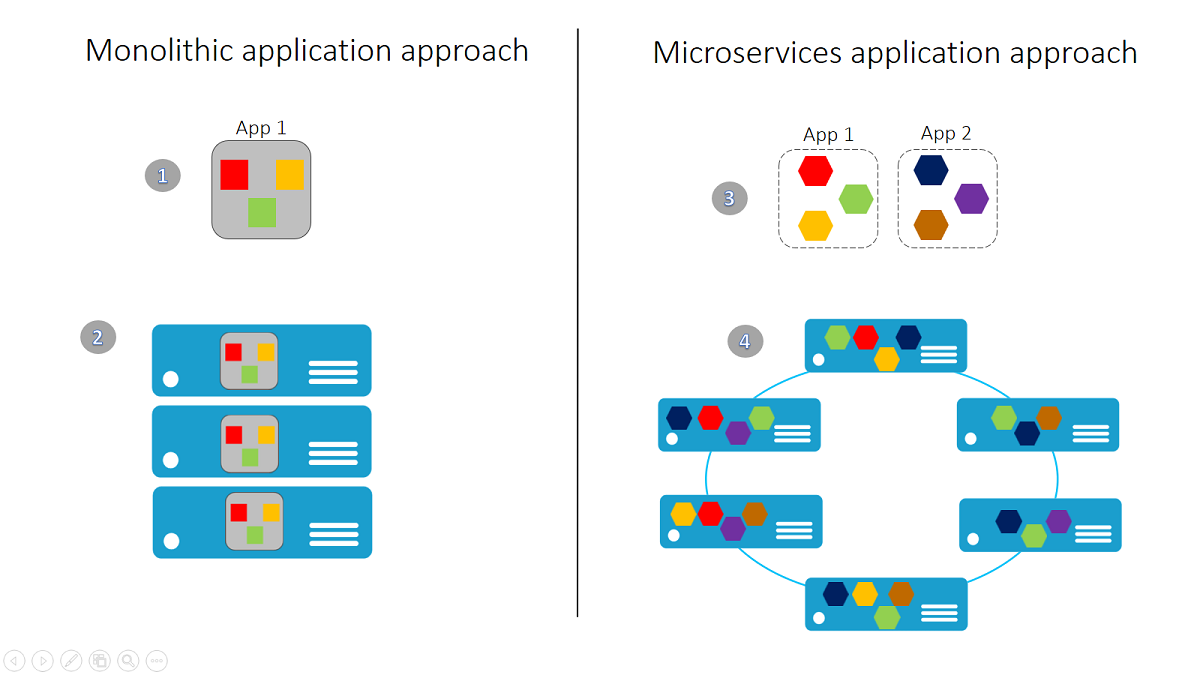
\includegraphics[width=\textwidth,keepaspectratio=true]{capitoli/imgs/monosvmicro.png}
	\caption{Il modello monolitico e i microservizi}
\end{figure}

\subsection{Vantaggi e svantaggi di un'architettura a microservizi}
Un'architettura di questo tipo porta con se ovviamente anche i suoi svantaggi e i suoi vantaggi. Sono proprio questi ultimi che la rendono molto adatta al Cloud Computing.

\subsubsection{Vantaggi}
\begin{itemize}
	\item  Velocità \\
	L'architettura a microservizi è quella che si sposa meglio con la metodologia agile. un microservizio deve avere sempre delle dimensioni ridotte e il suo sviluppo  dovrebbe avere una durata di circa due settimane. Ciò porta ad avere fin da subito piccole porzioni del sistema (i servizi appunto), pronte, testabili ed utilizzabili. Ogni microservizio inoltre è autonomo e può quindi giungere in ambiente di produzione indipendentemente dagli altri. In questo modo si riesce a reagire molto velocemente alle esigenze di mercato.
	
	\item Sperimentazione \\
	Con i microservizi la modularità del sistema è un notevole punto di forza. Sperimentare nuove tecnologie all'interno di un singolo microservizio ha un impatto nullo su tutti gli altri. Si è in questo modo molto più invogliati a ricercare sempre più nuove tecnologie da inserire nel proprio prodotto. Il rischio è minimo in quanto, anche nel caso l'esperienza risulti fallimentare, la mole di lavoro che comporta la modifica di un microservizio e veramente molto ridotta.
	
	\item Tecnologie ad hoc \\
	Altro fattore da considerare è la possibilità di differenziare le tecnologie a seconda del microservizio. Si prenda come esempio la vastità di database che sono disponibili all'uso. Un database che è appropriato per un microservizio potrebbe non essere la scelta migliore per un altro. 
	
	\item Scalabilità \\
	I software con un'architettura a microservizi sono pensati per scalare orizzontalmente in maniera estremamente agevole. Si possono replicare a piacimento tramite l'utilizzo di containers e hanno un comportamento distribuito anche nel caso si trovino sulla stessa macchina, in quanto i container li isolano da tutti gli altri.
	
	\item Facilità di Deployment \\
	Le modifiche hanno un impatto molto ridotto nell'interno sistema. Grazie a ciò è possibile rilasciare sul mercato il software aggiornato con frequenze molto maggiori. Potenzialmente ogni modifica può subito essere pubblicata e non occorre attenersi a lunghi processi di release in cui si cerca il più possibile di accumulare modifiche da effettuare per poi applicarle tutte insieme.
	
	\item Portabilità \\
	Il software a microservizi è facilmente componibile e portabile su più contesti e dispositivi, come web,mobile ma anche sistemi embedded o dispositivi indossabili ad esempio.	
\end{itemize}

\subsubsection{Svantaggi}
\begin{itemize}
	\item Dipendenza dalla rete \\
	E' questo il principale punto di critico di un'architettura a microservices. Abbiamo quanto l'interazione tra i singoli microservizi faccia affidamento su una comunicazione attraverso internet. Ovviamente questo deve essere un requisito fondamentale. In mancanza di una connessione adeguata tutto il sistema smette di funzionare.
	
	\item Identità e autenticazione \\
	Una volta che un utente del software effettua il login occorre garantire che la sua autenticazione, e soprattutto la sua identità, venga mantenuta in tutti i microservizi che andranno a comporre la sua esperienza utente.
\end{itemize}

\section{Containers}
I container sono l'habitat naturale dei microservizi. Essi forniscono al software tutto ciò che gli è necessario, garantendogli un ambiente estremamente leggero e flessibile.

\begin{figure}[h!]
	\centering
	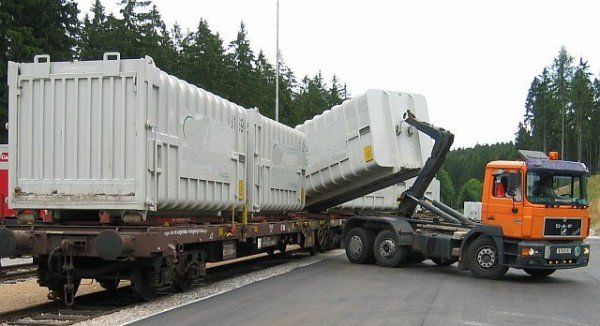
\includegraphics[width=\textwidth,keepaspectratio=true]{capitoli/imgs/spostamentocontainer.png}
	\caption{Containers nell'accezione dell'industria dei trasporti}
\end{figure}



\paragraph{}
Già la parola stessa container vuole alludere ad una analogia con l'attrezzatura specifica dei trasporti. Da dove è nata lì la necessità dell'utilizzo dei container? Immaginiamo lo scenario in cui alcune merci andassero trasportate prima via terra, magari con un camion, e poi via mare per raggiungere un altro stato. Prima dell'avvento dei container il camion arrivava al porto, andava aperto e il contenuto passato in un mercantile pronto sul molo. L'operazione era effettuata manualmente e i singoli imballaggi erano trasbordati uno alla volta con grande dispendio di tempo e mezzi. Si iniziò allora a considerare più pratica l'idea di trasbordare sulla nave l'intero corpo del camion. Nacquero così i container: contenitori multiuso, realizzati in formati standard che possono essere passati con facilità da un camion a una nave, poi magari su un treno merci e così via.

\paragraph{}
E così anche nel nostro caso abbiamo bisogno di uno strumento che possa contenere i microservizi e le applicazioni, che ci consenta di manovrarle con facilità senza sapere cosa facciano esattamente.
I containers sono infatti un metodo di virtualizzazione del sistema operativo che ha come obiettivo quello di isolare il software che ospita, permettendo di eseguire le applicazioni e le loro dipendenze in processi completamente isolati. L'infrastruttura del container interagisce direttamente con il kernel della macchina che lo ospita, scavalcando gli altri layer. In qualsiasi sistema operativo collochiamo il container, le sue configurazioni interne rimarranno sempre separate, e l'applicazione contenuta avrà garantito il suo ecosistema necessario all'esecuzione. Non ci si deve preoccupare, ad esempio, di produrre una versione software per Windows e una per sistemi UNIX, ma la soluzione a container e unica e portabile. 

\begin{figure}[h!]
	\centering
	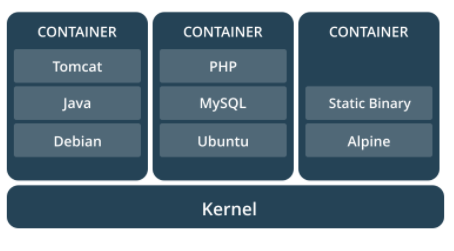
\includegraphics[width=\textwidth,keepaspectratio=true]{capitoli/imgs/container.PNG}
	\caption{Schematizzazione di tre container sulla stessa macchina ospitante}
\end{figure}

\subsection{I containers e le Macchine Virtuali}
Stando alla descrizione dei container che abbiamo dato fino a questo punto potrebbe sorgere una domanda: perché utilizzare i container se potrebbero essere usate delle macchine virtuali? Una Virtual Machine è per sua natura già isolata dalla macchina che la ospita. La risposta sta nella leggerezza d'uso dei container. I container infatti non virtualizzano l'hardware della macchina, ma solamente il layer applicativo, rendendoli più portabili ed efficienti.

\paragraph{}
Non avendo un proprio sistema operativo, il peso di un container e dell'ordine di qualche Megabyte, contro i Gigabyte di una macchina virtuale che sovrappone il proprio sistema operativo a quello della macchina ospitante. A differenza delle macchine virtuali inoltre, i container non necessitano dell'Hypervisor, un componente che svolge delle attività di controllo e coordinamento sulle macchine virtuali. 

\begin{figure}[h!]
	\centering
	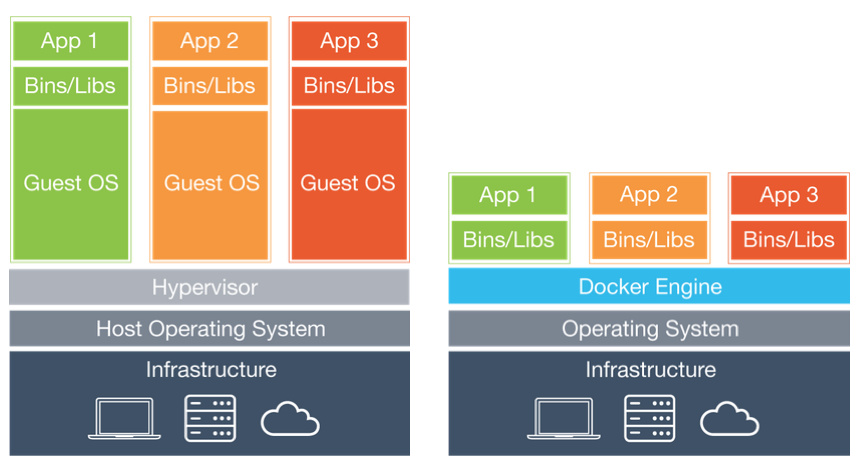
\includegraphics[width=\textwidth,keepaspectratio=true]{capitoli/imgs/ContainersvsVms.PNG}
	\caption{Confronto tra macchine virtuali e container, nell'esempio con l'utilizzo di un Docker Engine}
\end{figure}

\subsection{Vantaggi dei container}
Andiamo a ricapitolare quali sono le principali motivazioni che possono spingerci all'adozione dei container.
\begin{itemize}
	\item Coesione dell'ambiente \\
	L'ambiente di un container è fortemente disaccoppiato dalla macchina in cui si trova. Questo fa si che il proprio contenuto sia facilmente replicabile e portabile ovunque.
	
	\item Gestione delle risorse \\
	Con i containers si ha una gestione delle risorse di calcolo molto più efficiente. Richiedendo poche risorse alla macchine ospitante, si ha la possibilità di eseguire molti più container contemporaneamente. 
	
	\item Produttività \\
	Diminuendo le dipendenze, ci si alleggerisce di tutta la mole di lavoro necessaria per configurare correttamente un prodotto. 
	
	\item gestione degli aggiornamenti. \\
	Molto spesso la gestione degli aggiornamenti è un meccanismo già compreso nei container engine, come Docker.
\end{itemize}

\subsection{I container e i microservizi}
Possiamo quindi comprendere come i container siano estremamente appropriati ad ospitare del microservizi. Ponendo un microservizio dentro ogni container, abbiamo la garanzia che ogni microservizio operi come un sistema separato, anche nell'eventualità che due servizi risiedano nella stessa macchina fisica. Ogni microservizio inserito in un container gode automaticamente di tutti i vantaggi di portabilità e flessibilità che sono tra i requisiti fondamentali che ci spingono verso l'architettura a microservizi.

\subsection{Docker}

\begin{figure}[h!]
	\centering
	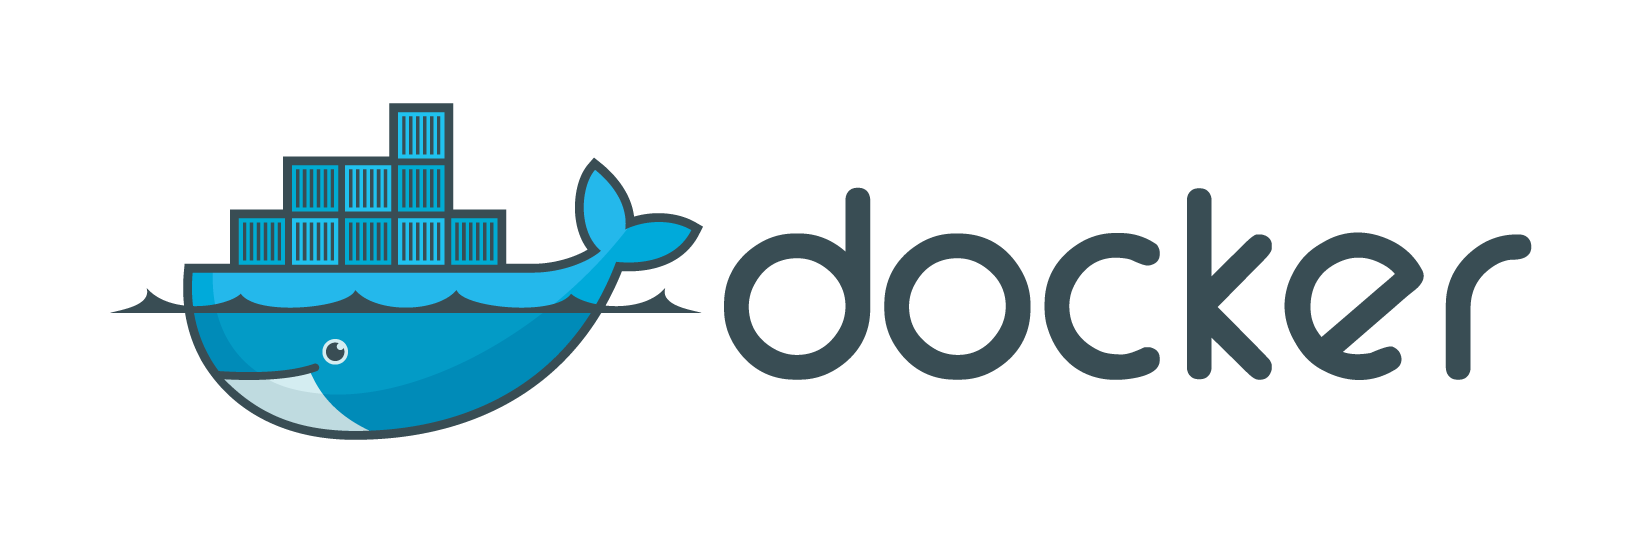
\includegraphics[width=\textwidth,keepaspectratio=true]{capitoli/imgs/docker.png}
	\caption{Logo di Docker}
\end{figure}

\paragraph{}
Docker è una piattaforma open source nata nel 2013 e scritta in linguaggio Go. Il suo scopo è quello di facilitare ed automatizzare il deployment delle applicazioni all'interno dei container. Il tool offre allo sviluppatore delle comode API di gestione che consentono agli sviluppatori di testare le applicazioni, effettuare build e distribuire il proprio prodotto. Docker fa utilizzo di numerose librarie come, ad esempio, libcontainer che ha lo scopo di interagire con il kernel di Linux.  In questo modo, isolando risorse, servizi e processi, dalla prospettiva dell'utilizzatore del container si ha l'impressione di un utilizzo esclusivo del sistema operativo.

\paragraph{}
Il contiene diviene con Docker così l'unità di distribuzione del prodotto. Quando il servizio è stato correttamente implementato, è pronto per essere distribuito e, attraverso il container, può essere inserito in un orchestratore per garantirne il ciclo di vita.

\paragraph{Docker Engine}
L'Engine di Docker è una struttura a strati, troviamo:
\begin{itemize}
	\item Il server, un demone chiamato dockerd che è sempre in running. E' il componente che maneggia gli oggetti Docker.
	\item Le REST API, che rappresentano l'interfaccia per interrogare il server.
	\item La Command Line Interface, che è quella con la quale si interfaccia l'utente e si aggancia alla REST API.
\end{itemize}

\begin{figure}[h!]
	\centering
	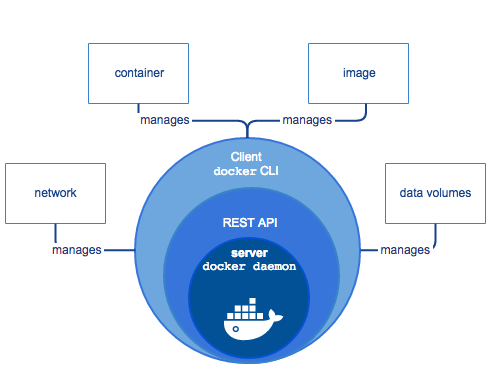
\includegraphics[width=\textwidth,keepaspectratio=true]{capitoli/imgs/dockerThinking.png}
	\caption{Docker engine}
\end{figure}

\paragraph{Architettura di Docker}
L'architettura di Docker è la classica architettura client-server. Il client parla direttamente con il Docker deamon che si trova sul server. E' proprio il dockerd che si prende l'onere di fare gran parte del lavoro, quello di far partire e distribuire i container.
\begin{figure}[h!]
	\centering
	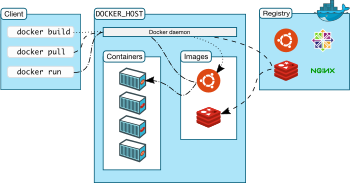
\includegraphics[width=\textwidth,keepaspectratio=true]{capitoli/imgs/architecturedocker.png}
	\caption{Architettura di Docker}
\end{figure}
\paragraph{}
I componenti che vanno a costituire l'architettura di Docker sono i seguenti:
\begin{itemize}
	\item Docker deamon \\
	Dockerd è in ascolto di chiamate da parte della REST API. E' sua responsabilità far funzionare tutto l'engine della gestione dei container.
	\item Docker client \\
	Lo scopo principale del client è interagire con chi sviluppa il contenuto dei container. Questo componente recepisce i comandi da parte dello sviluppatore e li traduce in chiamate per il deamon.
	\item Docker registries \\
	E' un registro che consente di conservare le immagini di Docker. Immaginiamo che sia interesse di chi li sviluppa poter conservare e mettere in vendita servizi implementati all'interno dei container. Vengono offerte anche delle comode API e uno store nel quale mettere in mostra le proprie immagini.
	\item  docker objects \\
	In questa categoria rientrano più tipologie di oggetti Docker, come quelli che andiamo ad analizzare qui di seguito.
	\item  Images \\
	un immagine è un template standard di sola lettura che si utilizza per parametrizzare un nuovo container che si sta per mettere in piedi. Per creare la propria immagine  con i parametri personalizzati, si dichiarano nel Dockerfile gli step necessari. Successivamente ad ogni step corrisponderà a un layer del container.
	\item  Container \\
	Un container è proprio l'istanziazione di una immagine, è infatti definito univocamente dalla propria immagine. E' un elemento che può essere gestito a piacimento e può essere collegato ad una o più reti, fattore importantissimo per far interagire il proprio contenuto con quello di altri container.
	\item Services \\
	I servizi permettono di scalare i container attraverso più Docker deamon. In questo modo si riesce a dare ugualmente l'impressione all'utente di utilizzare comunque un servizio esclusivo e centralizzato.
\end{itemize}



\subsection{Un'esuberante}
\begin{figure}[h!]
	\centering
	
\includegraphics[width=\textwidth,keepaspectratio=true]{capitoli/imgs/kubernetes_full.png}
	\caption{Logo di Un'esuberante}
\end{figure}

\paragraph{}
Abbiamo appena tessuto le lodi di Docker. Ora però poniamoci alcune domande: come possono essere coordinati, distribuiti e gestiti i container e il loro workload, man a mano che vengono consumate le risorse disponibili nell'infrastruttura sottostante? Come operano i container in un ambiente network multi-tenant? Quale livello di sicurezza propone Docker? E chi decide quale sia il giusto livello di astrazione?

\paragraph{}
Per far fronte a queste necessità è nato da Google nel 2014 Kubernetes. Esso offre un layer di astrazione per migliorare le performance dei container stessi eliminando molti dei processi manuali coinvolti nel deployment e nella scalabilità di applicazioni containerizzate. Consente di far cooperare opportunamente insiemi di container componendo delle unità logiche utili nelle nostre applicazioni.

\paragraph{Perché utilizzare Kubernetes?}
Le applicazioni di produzione si espandono su più container, che devono essere distribuiti su più server host. Kubernetes ti offre le capacità di orchestrazione e gestione necessarie per distribuire i container, in modo scalabile, al fine di gestire i carichi di lavoro. L'orchestrazione di Kubernetes consente di creare servizi applicativi che si estendono su più container, programmare tali container in un cluster, gestirne la scalabilità e l'integrità nel tempo.

\begin{figure}[h!]
	\centering
	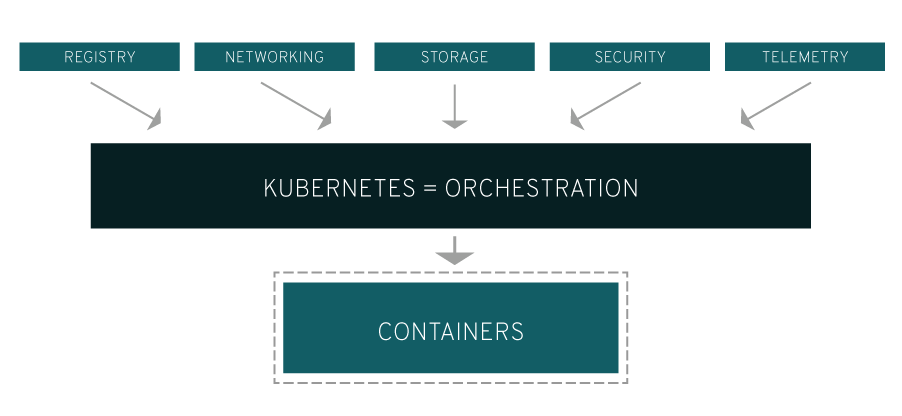
\includegraphics[width=\textwidth,keepaspectratio=true]{capitoli/imgs/kubernetes-diagram.png}
	\caption{Ruolo di orchestratore di Kubernetes}
\end{figure}

\paragraph{I Pod di Kubernetes, cosa sono?}
Kubernetes risolve molti dei noti problemi relativi alla proliferazione dei container, raggruppandoli in un Pod. I pod aggiungono quindi un livello di astrazione ai cluster di container. La loro funzione è quella di alleggerire i carichi di lavoro e fornire i servizi necessari, tra cui rete e storage, ai container stessi. Kubernetes agevola, inoltre, il bilanciamento del carico all'interno dei pod e garantisce l'utilizzo di un numero di container adeguato per supportare i tuoi carichi di lavoro.

\paragraph{Architettura di Kubernetes}
\begin{figure}[h!]
	\centering
	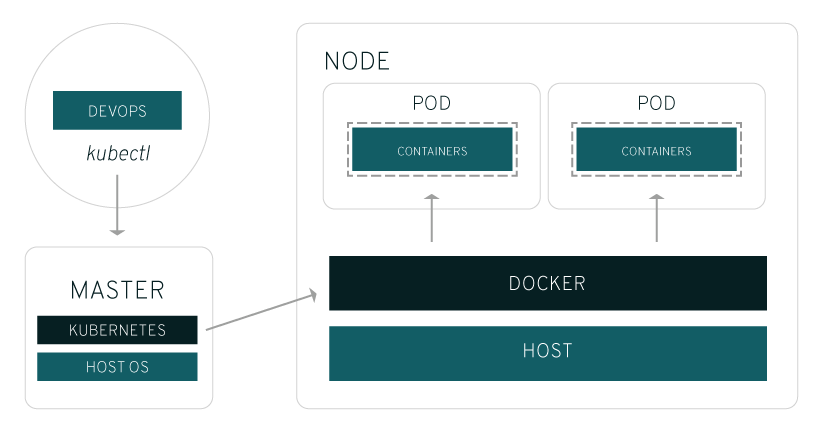
\includegraphics[width=\textwidth,keepaspectratio=true]{capitoli/imgs/kubernetesarchitetcture.png}
	\caption{Architettura di Kubernetes}
\end{figure}

Andiamo a definire quelli che sono i termini di riferimento in Kubernetes:
\begin{itemize}
	\item Master \\
	E' la macchina che controlla i nodi Kubernetes. È il punto di origine di tutte le attività assegnate.
	\item Nodi \\
	Queste macchine eseguono le attività assegnate richieste. Sono controllate dal nodo master di Kubernetes. Possono essere assimilate con gli host dei container.
	\item Pod \\
	Rappresenta un gruppo di uno o più container distribuiti su un singolo nodo. Tutti i container presenti in un pod condividono indirizzo IP, IPC, nome host ed altre risorse. I pod astraggono la rete e lo storage dal container sottostante, consentendo di spostare i container nei cluster con maggiore facilità.
	\item Servizio \\
	Questa componente ha la funzionalità di disaccoppiare le definizioni del lavoro dai pod. I proxy di servizio di Kubernetes ricevono automaticamente le richieste di servizio al pod corretto, indipendentemente dagli spostamenti nel cluster, anche nel caso in cui esso sia stato riposizionato.
	\item Kubelet \\
	Questo servizio viene eseguito sui nodi, legge i manifest del container e garantisce che i container definiti vengano avviati ed eseguiti.
	\item Kubctl \\
	Questo componente si interfaccia direttamente con il programmatore. Presenta una riga di comando per la creazione e gestione dei pod.
\end{itemize}

\paragraph{E Docker?}
La piattaforma docker mantiene le proprie funzioni. Quando Kubernetes assegna un pod ad un nodo, il kubelet su quel nodo chiede a docker di lanciare i container specificati. Quindi, il kubelet legge continuamente lo stato di quei container da docker e aggrega le informazioni nel nodo master. Docker invia i container sul nodo, avvia e arresta normalmente i container. La differenza è che un sistema automatizzato con Kubernetes chiede a docker di eseguire queste operazioni, anziché assegnarle ad un amministratore, il quale deve eseguirle manualmente su tutti i nodi, in tutti i container.

\section{Multitenancy}
La multitenancy è un paradigma che, andando a braccetto con il cloud computing, si sta diffondendo sempre di più nel panorama delle architetture software. Esso prevede che una singola istanza del software in questione, situato su un server, sia utilizzato da molti utenti, chiamati tenant. I tenant condividono l'accesso comune al servizio con privilegi differenziati sulle istanze software. L'obiettivo principale è quello di garantire scalabilità al servizio e dare al tenant la percezione di un possesso esclusivo del software.

\paragraph{Vantaggi della Multitenancy}
\begin{itemize}
	\item Costi \\
	Scalare un'architettura multitenant è più economico, in quanto si interviene solamente in un'unica macchina fisica e acquistare hardware più performante risulta meno dispendioso. Inoltre in questo modo si riduce anche il numero di licenze da acquistare, nel caso siano necessarie, il che può comportare un notevole risparmio.
	\item Data Mining \\
	Nel caso sia necessario estrapolare dei dati da tutti i clienti, avere dei tenant tutti sulla stessa macchina rende l'operazione molto più immediata.
	\item  Release Management \\
	Al rilascio di una nuova versione il processo risulta essere molto semplificato. Ciò viene ovviamente dal fatto che dovendo aggiornare una sola istanza del software su una sola macchina fisica la mole di lavoro è sicuramente minore.
\end{itemize}

\paragraph{Requisiti}
Ovviamente un'architettura multitenant ha anche dei requisiti. Sicuramente, nonostante l'unicità del software, si deve garantire un alto grado di "personalizzazione" ai diversi tenant, proprio come se avessero un utilizzo esclusivo del servizio. Da un altro lato ci si aspettano elevati parametri di security, robustezza e prestazioni.

\section{Monitoring Tools}
La centralizzazione portata dal SaaS comporta anche un radicale cambiamento delle modalità di monitoring del sistema. Non è pensabile che una persona possa andare a controllare tutti i log dei servizi e misurare le prestazioni degli stessi manualmente. E' necessario l'utilizzo di appositi tool che hanno come finalità quella di raccogliere questa mole di informazioni, elaborarle e presentarle al personale addetto del provider nel modo più intellegibile possibile. In questa ottica andiamo a presentare due tool utilizzati nel progetto: Prometheus e Grafana.
\subsection{Prometheus}
\begin{figure}[h!]
	\centering
	
\includegraphics[width=0.5\textwidth,keepaspectratio=true]{capitoli/imgs/prometheuslogo.png}
	\caption{Logo di Prometheus}
\end{figure}
\paragraph{}
prometheus è un tool di monitoring open-source nato nel 2012 e scritto in Go. Si adatta sia alle architetture centralizzate che a quelle distribuite. La struttura del tool e pensata per garantire un validissimo supporto nel caso il servizio monitorato abbia dei malfunzionamenti. Vediamo un elenco delle caratteristiche principali.
\begin{itemize}
	\item Un data model multidimensionale che ha lo scopo di raccogliere tutti i dati
	\item Un query language flessibile per far fronte a questi dati
	\item Engine per la rielaborazione dei dati
	\item Meccanismi sofisticati per collezionare serie storiche
	\item Supporto per le dashboard
\end{itemize}
\subsection{Grafana}
\begin{figure}[h!]
	\centering
	
\includegraphics[width=0.3\textwidth,keepaspectratio=true]{capitoli/imgs/grafanalogo.png}
	\caption{Logo di Grafana}
\end{figure}
Grafana consente di avere un portale centralizzato da cui monitorare tutti i servizi. Consente di visualizzare dati, creare degli alert e visualizzare tutte le informazioni in comode interfacce per gli utenti.
\begin{figure}[h!]
	\centering
	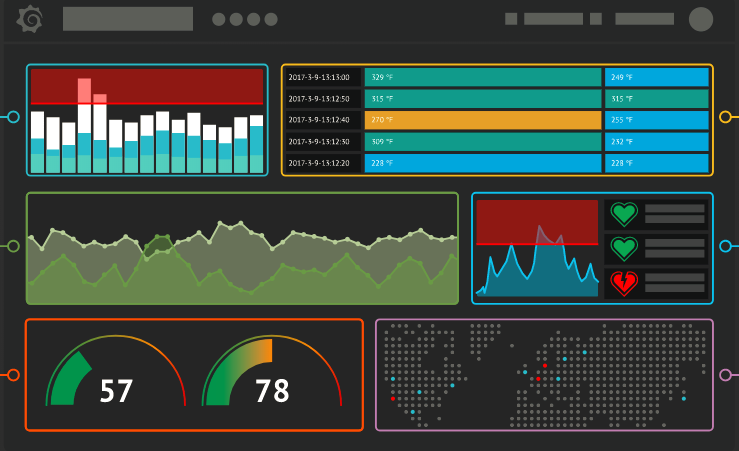
\includegraphics[width=0.7\textwidth,keepaspectratio=true]{capitoli/imgs/grafanainterface.PNG}
	\caption{Una delle interfacce di Grafana}
\end{figure}

\section{BlueMix Services}
\begin{figure}[h!]
	\centering
	
\includegraphics[width=0.7\textwidth,keepaspectratio=true]{capitoli/imgs/bluemixlogo.png}
	\caption{Logo di IBM BlueMix}
\end{figure}
Come abbiamo accennato precedentemente, IBM BlueMix è una PaaS che offre molti microservizi utili per il cloud computing. Il vantaggio dei microservizi è proprio questo, possono essere utilizzati a piacimento in qualsivoglia progetto. Alcuni dei servizi BlueMix sono stati anche utilizzati nel nostro progetto e altri lo saranno in seguito, con degli sviluppi futuri.
\paragraph{}
Ne sono un esempio il database DB2 e Kubernetes, che nel nostro caso sono stati proprio integrati nelle loro versioni presenti su BlueMix. E' possibile inoltre che in futuro si adotti un'altro database IBM sempre presente su BlueMix, Cloudant, un database NoSQL nativo cloud.
